% Template for ICIP-2010 paper; to be used with:
%          spconf.sty  - ICASSP/ICIP LaTeX style file, and
%          IEEEbib.bst - IEEE bibliography style file.
% --------------------------------------------------------------------------
\documentclass{article}
\usepackage{spconf,amsmath,graphicx}
\usepackage{algorithm}
\usepackage{algorithmicx}
\usepackage{algpseudocode}


% Example definitions.
% --------------------
\def\x{{\mathbf x}}
\def\L{{\cal L}}

% Title.
% ------
\title{EFFICIENT BOUNDARY VECTORIZATION ON NOISY RASTER IMAGES}
%
% Single address.
% ---------------
\name{Weihong Li}
\address{The Graduate Center of the City University of New York, \\
         Dept of Computer Science\\
	 365 Fifth Ave., New York, NY, 10016 USA}
%
% For example:
% ------------
%\address{School\\
%	Department\\
%	Address}
%
% Two addresses (uncomment and modify for two-address case).
% ----------------------------------------------------------
%\twoauthors
%  {A. Author-one, B. Author-two\sthanks{Thanks to XYZ agency for funding.}}
%	{School A-B\\
%	Department A-B\\
%	Address A-B}
%  {C. Author-three, D. Author-four\sthanks{The fourth author performed the work
%	while at ...}}
%	{School C-D\\
%	Department C-D\\
%	Address C-D}
%

\newcommand{\Eq}[1] {Eq.~(\ref{eq:#1})}
\newcommand{\Fig}[1]{Fig.~\ref{fig:#1}}
\newcommand{\Sec}[1]{Sec.~\ref{sec:#1}}
\newcommand{\Eqs}   {Eqs.~}
\newcommand{\Figs}  {Figs.~}
\newcommand{\Tbl}[1]{Table~\ref{tbl:#1}}
\newcommand{\Etal}  {{\it et al.}}
\newcommand{\Figa}[1]{Fig.~\ref{fig:#1}(a)}
\newcommand{\Figb}[1]{Fig.~\ref{fig:#1}(b)}
\newcommand{\Figc}[1]{Fig.~\ref{fig:#1}(c)}
\newcommand{\Figd}[1]{Fig.~\ref{fig:#1}(d)}
\newcommand{\Fige}[1]{Fig.~\ref{fig:#1}(e)}
\newcommand{\Figf}[1]{Fig.~\ref{fig:#1}(f)}
\newcommand{\Figg}[1]{Fig.~\ref{fig:#1}(g)}
\newcommand{\Figh}[1]{Fig.~\ref{fig:#1}(h)}
\newcommand{\Figi}[1]{Fig.~\ref{fig:#1}(i)}

\graphicspath{{figures/}{experiments/}}


\begin{document}
%\ninept
%
\maketitle
%
\begin{abstract}
The problem considered here is boundary vectorization
for noisy binary images. The difficulty of the problem lies in
outliers and holes of non-perfect images. A general framework based
on an adaptive 2D ball-pivot algorithm (BPA) is proposed to efficiently suppress
the noisy, fill holes and generate contours for those images.
The contribution of this work is to solve the boundary vectorization problem for noisy binary images
by proposing an fast algorithm with the time and space complexity of $O(n)$.
The potential applications of this method include medical
image processing, 3D point cloud data modeling, object tracking, etc.
\end{abstract}
%
\begin{keywords}
image processing, raster image, 3D modeling, geometry compression
\end{keywords}
%
\section{INTRODUCTION}
\label{sec:intro}


There exists numerous works on boundary vectorization,
such as those described in \cite{DP_RP,DP_LC,DP_AAKMT}.
However, these approaches
only consider the cases where perfect raster image data is provided.
For non-perfect data, these proposed methods were failed in various cases.
The problem considered here is to compute contours
for non-perfect binary images which may contain holes
along the boundary as well as noise or outliers
inside the boundary. Here, {\it boundary} refers to the
out-most region of any raster image and
{\it contour} refers to a vectorized boundary.


The Douglas-Peucker (DP) algorithm \cite{DP_DP} is widely used
to compute boundary vectorization for binary images.
Although  with the improvement of implementation described in \cite{DP_HS, DP_HS94},
the complexity of this approach is of $O(nlogn)$, this method cannot fill the
holes of the noisy data or handle the case
where spurious interior points are presented.
Agarwal et al. \cite{DP_AV} considered the problem of
approximating a polygon chain using another one to minimize the number of
vertices. However, for a raster image, the vertices
defining the contour were not known.
For example, \Figa{failed_case} shows a binary cross-section
image of a 3D point cloud data of a building. \Figb{failed_case} shows
the contour generated from DP algorithm. The problem is that there are
a lot of holes along the contour and the noise data inside of the
boundary are modeled inappropriately.
To tackle these issues, a general boundary vectorization framework is proposed
based on ball-pivoting algorithm (BPA) \cite{BPA_BMRS} which was used
originally on 3D point cloud data process to generate 3D mesh representation.
\Figc{failed_case} shows
the contour computed by the proposed framework which fills holes between gaps
and suppresses noise inside the boundary.


\begin{figure*}[hbtp]
\begin{center}
\begin{tabular}{cc}
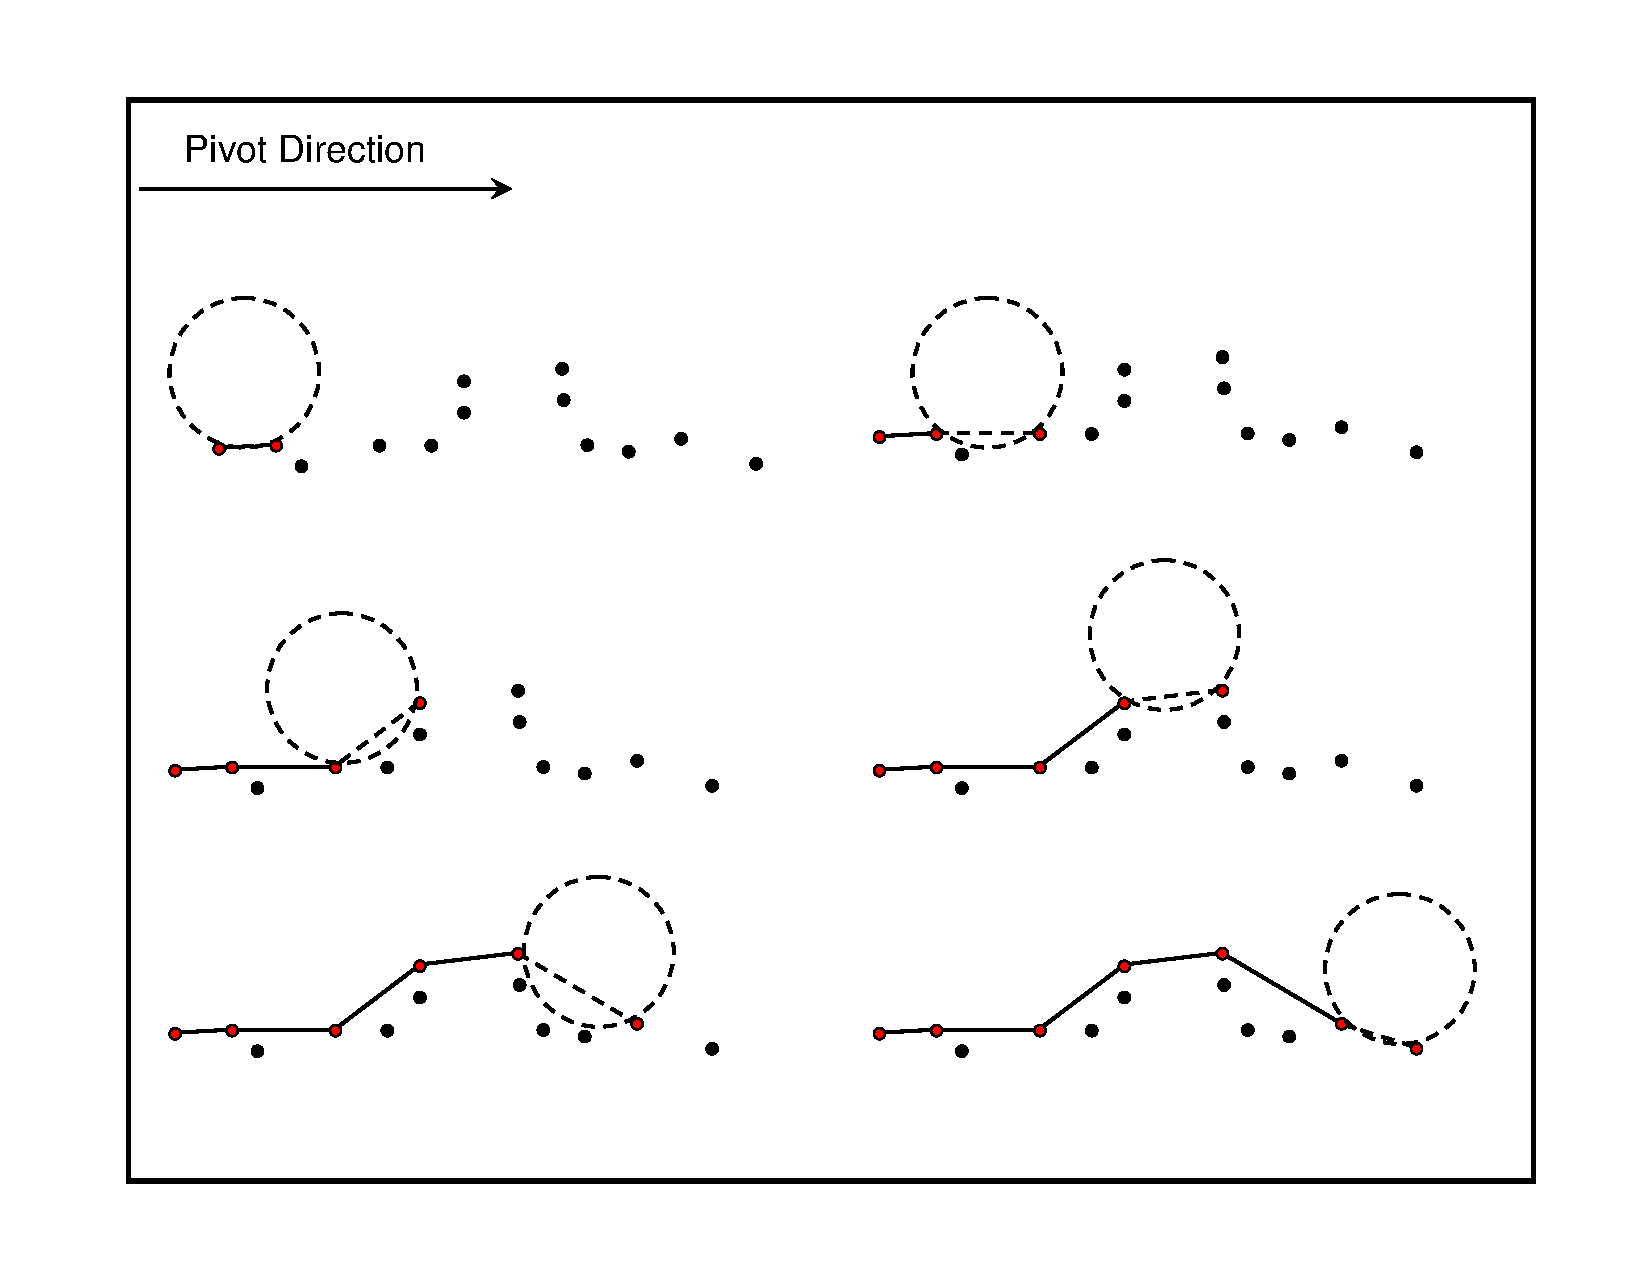
\includegraphics[width=0.48\textwidth]{figures/BPA_init.pdf} &
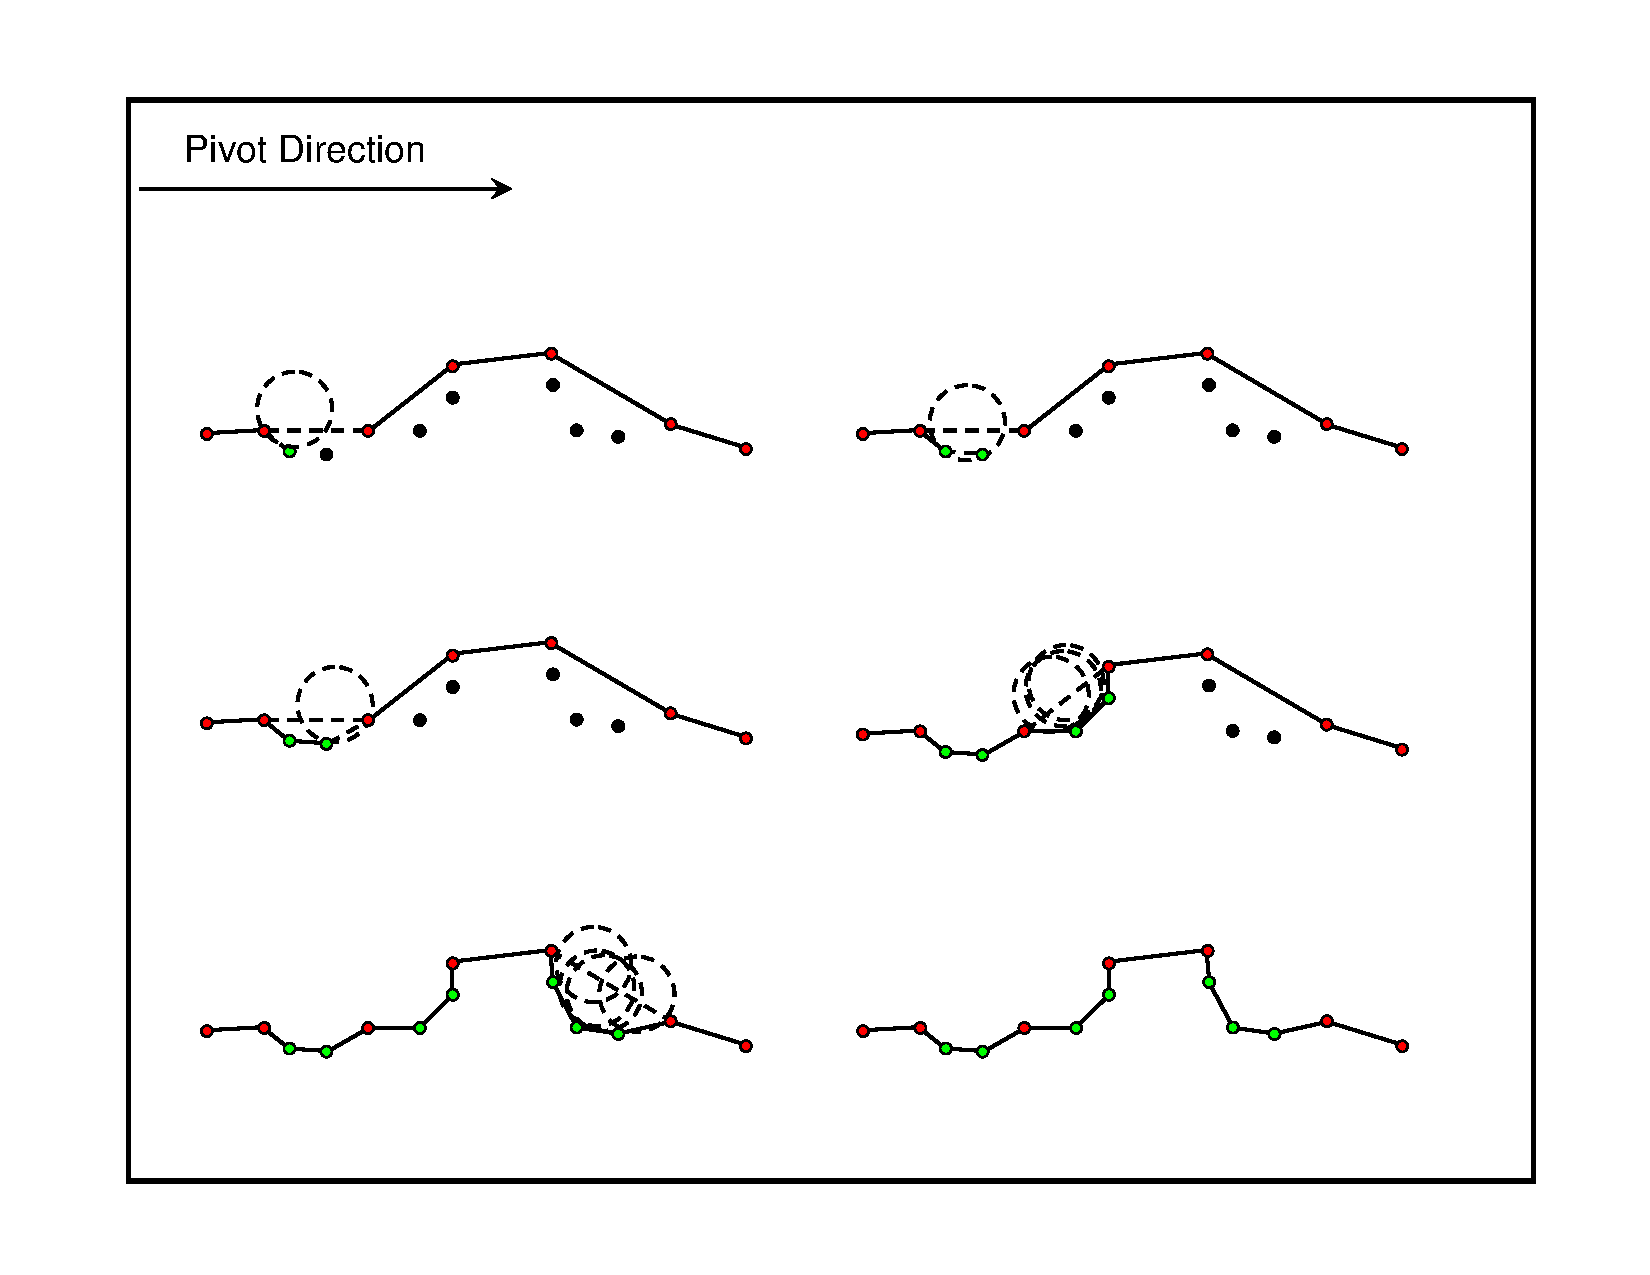
\includegraphics[width=0.48\textwidth]{figures/BPA_refine.pdf} \\
(a) & (b)
\end{tabular}
\end{center}
\caption{Adaptive ball pivoting algorithm:
(a) Initial pivoting with a ball of radius 2$r$;
(b) Refinement with a ball of radius $r$.}
\label{fig:BPA}
\end{figure*}


The idea of the BPA is straight-forward:
pivot a ball on a starting point in the image
until it touches another data point as depicted in \Figa{BPA}.
Add the new touched
data point into an ordered list as the vertices of the contour polygon and
set it as the new pivoting point.
Keep doing this pivoting process until all data points are touched.

\section{Boundary Vectorization}
The basic idea behind the proposed framework for contour computation is as follows:
apply BPA on a selected starting point until
either the ball pivots back to the starting point which indicates a closed boundary is detected,
or the ball reaches a gap which means this contour is a non-closed
contour and one of the end points is reached.
Because the ball can start pivoting along either clock-wise direction or counter clock-wise direction,
another pivoting process at start pivoting from the other direction is conducted.
When both directions have been explored, a contour computation is done.
After this, the refinement process is carried out for each line segments using the same BPA algorithm.
For this refinement, the starting point is now the first end point of a line
and the stopping case is that the ball reaches the other point or it
reaches a gap.

Here is more detailed description for the algorithm.
At the initial BPA stage, a relatively large radius $r$ is chosen as a coarse step to cover all gaps between data points.
The output of the initial BPA, $\boldsymbol{\Phi}$, contains an ordered list of the boundary data
points $\boldsymbol{P}$ and their corresponding directions $\overrightarrow{\boldsymbol{R}}$ in which
the ball $C$ starts pivoting.
The BPA refinement process applies a smaller radius, say $r' = r/2$,
to $\boldsymbol{\Phi}$ to get more accurate results, as shown in \Figb{BPA}.
For this stage, the length of each line segment formed by adjacent points is checked,
$\ell = \overline{P_0P_1}$, in $\boldsymbol{\Phi}$.
For long line segments, the BPA is applied between the two adjacent points.
When the ball reaches the second end point, a new list of ordered boundary points,
$\boldsymbol{\Phi'}$, is inserted into $\boldsymbol{\Phi}$ between $P_0$ and
$P_1$.
This process continues until it finishes checking every adjacent point in $\boldsymbol{\Phi}$.
The refinement stops when $r'$ falls below threshold $\tau_r$.

The key parameter for the BPA algorithm to work successfully is finding
a good initial size of the ball for pivoting.
Here are some general guidances for choosing the radius. If a contour is known to be a closed polygon,
the initial radius should be big, e.g. the width of an image, to cover all gaps along the boundary.
Otherwise, if a boundary consists of sub-boundaries, one could select a relative small radius to start.

An example on the proposed framework is shown in \Fig{BPA_refinement}.
The initial BPA takes radius $\tau_r$ = 128,
which produced a coarse contour as shown in \Figa{BPA_refinement}.
\Figb{BPA_refinement} - \Figd{BPA_refinement} show that the contour is becoming more
accurate as the radius $\tau_r$ decreases from 32 to 2. Note that the original
image size is 1024x392 pixels as shown in \Figa{failed_case}.

\begin{figure}[htbp]
\begin{center}
\begin{tabular}{cc}
\fbox{
\includegraphics[width=0.22\textwidth]{global_init_refine_with_rad_128.png}} &
\fbox{
\includegraphics[width=0.22\textwidth]{global_init_refine_with_rad_32.png}} \\
(a) & (b) \\
\fbox{
\includegraphics[width=0.22\textwidth]{global_init_refine_with_rad_8.png}} &
\fbox{
\includegraphics[width=0.22\textwidth]{global_init_refine_with_rad_1.png}} \\
(c) & (d)
\end{tabular}
\end{center}
\caption{Boundary vectorization of a binary image with (a) radius = 128
(b) radius = 32 (c) radius = 8 (d) radius = 2.}
\label{fig:BPA_refinement}
\end{figure}




%%%%%%%%%%%%%%%%%%%%%%%%%%%%%%%%
%%%%%%   Complexity %%%%%%%%%%%%
%%%%%%%%%%%%%%%%%%%%%%%%%%%%%%%
\subsection{Complexity Analysis}
\label{sec:CA}

\begin{algorithm}
\caption{The 2D Adaptive Ball-Pivot Algorithm}
\label{alg.ABPA}
\begin{algorithmic}[1]
\Procedure {ABPA}{$I$, $W$, $\boldsymbol{\Phi}$}
\State $r \leftarrow W$
\State $P_i \leftarrow S(I) $ \Comment{compute the $seed$ point}
\While {$P_i \notin \boldsymbol{\Phi} \: \land  \: !isGap(\boldsymbol{\Phi}, P_i)$}
   \State $Append(\boldsymbol{\Phi}, P_i)$
   \State $P_i \leftarrow pivotBall(\boldsymbol{\Phi}, I, r)$ \Comment{regular 2D BPA}
\EndWhile

\While {$r > \epsilon$} \Comment {iterative BPA refinement}
   \State $r \leftarrow r/2$
   \For { each line $\overline{P_iP_j} \in \boldsymbol{\Phi} $}
      \State $\boldsymbol{L'} \leftarrow \emptyset$, $P_k \leftarrow P_i$
      \While {$P_k \ne P_j  \: \land  \: !isGap(\boldsymbol{L'}, P_k)$}
         \State $Append(\boldsymbol{L'}, P_k)$
         \State $P_k \leftarrow pivotBall(\boldsymbol{L'}, I, r)$
      \EndWhile
      \If { $P_k = P_j $ }
         \State $Substitute(\boldsymbol{\Phi}, P_i, P_j, \boldsymbol{L'})$
      \EndIf
   \EndFor
\EndWhile
\EndProcedure
\end{algorithmic}
\end{algorithm}

The 2D adaptive ball-pivot algorithm is summarized in Algorithm \ref{alg.ABPA}.
The function $S()$ is to randomly pick up a starting point, which
is only $O(1)$ complexity. The $Append()$ function is to concatenate the vertex
points, which is also $O(1)$. The regular 2D ball-pivot algorithm, $BPA()$,
carries out the geometry computation on each pivot point based on the size of the
radius of the ball. Basically, for each pivoting, the area
in the image covered by this operation is checked. If there is a data point in
this area, the pivoting operation ends for the current pivoting point.
Because the minimum angle for each pivoting in the computation is set to be 1 degree,
the worst case for the whole 2D $BPA()$ algorithm is $O(360*n) = O(n)$

For the refinement process, each line $\overline{P_iP_j}$ of the contour generated
in the previous iteration is checked using the same algorithm in $BPA()$. This only
takes $O(n)$ time for computation. The $Substitute()$ function inserts extra
points between two adjacent vertices, and $isGap()$ function carries out simple algebra computation.
The complexity for both operations is $O(1)$.
Because the round of the refinement process is bounded by a predefined constant
number, say $C$, the complexity of this refinement is also bounded by $O(C*n) = O(n)$.

The implementation of the BPA uses $O(m)$ memory space, where $m$ is the size of the 2D image.
This complexity includes the enque/dequue the vertex points of the boundary, the
pivoting geometry computation and the $Substittue()$ and $isGap()$ computations.

\begin{figure*}[htbp]
\begin{center}
\begin{tabular}{ccc}
\fbox{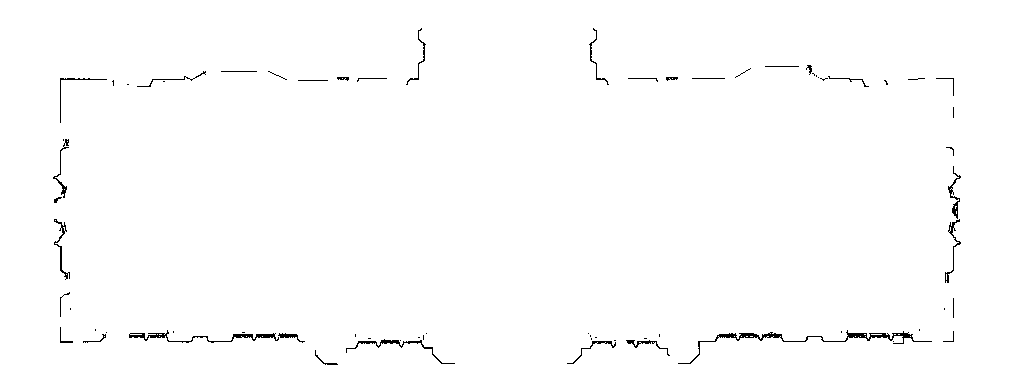
\includegraphics[width=0.3\textwidth]{failed_case.png}} &
\fbox{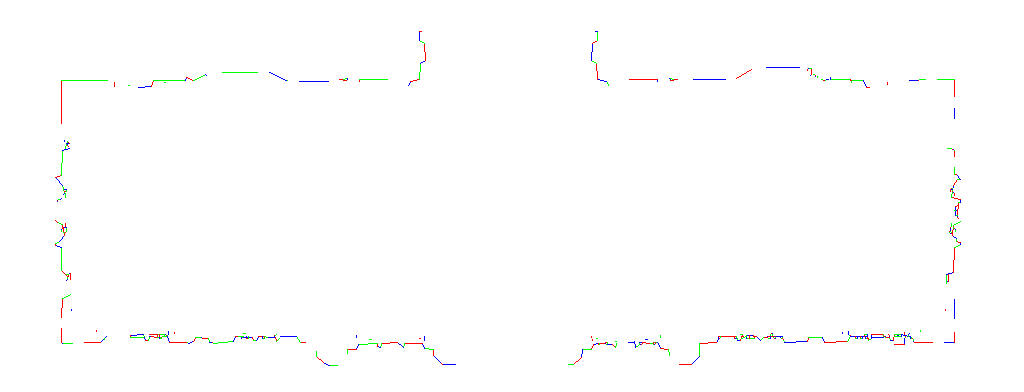
\includegraphics[width=0.3\textwidth]{failed_case_ply.png}} &
\fbox{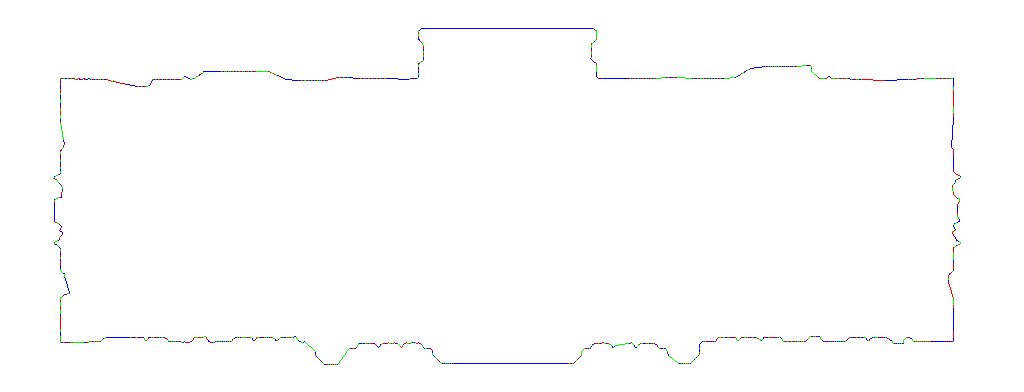
\includegraphics[width=0.3\textwidth]{failed_case_bpa.png}} \\
(a) & (b) & (c)
\end{tabular}
\end{center}
\caption{(a) An example of binary image.
(b) The vectorization result based on DP algorithm and
(c) The vectorization result from proposed BPA algorithm.}
\label{fig:failed_case}
\end{figure*}

\begin{figure*}[htbp]
\begin{center}
\begin{tabular}{ccc}
\fbox{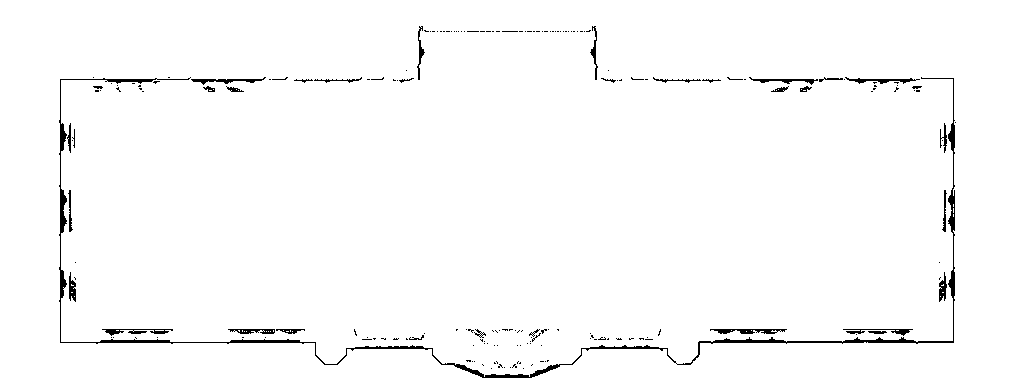
\includegraphics[width=0.3\textwidth]{aaa_image_slice_0529.png}} &
\fbox{
\includegraphics[width=0.3\textwidth]{bbb_image_slice_1024_392_0533_refine_with_rad_1_and_merged.png}} &
\fbox{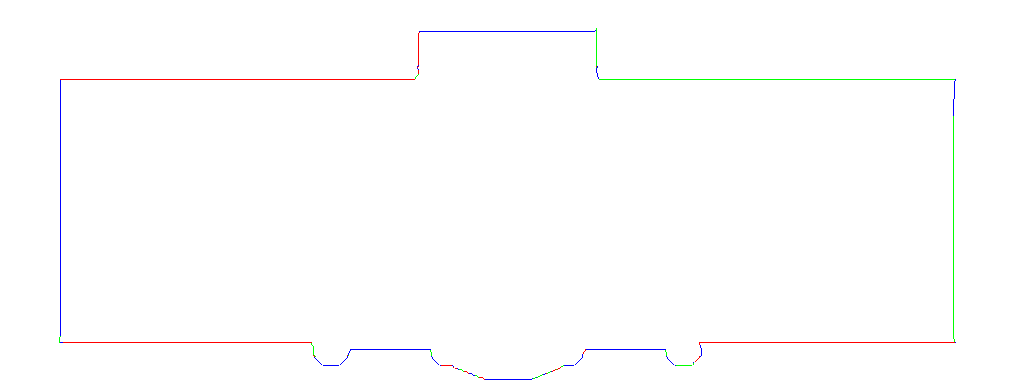
\includegraphics[width=0.3\textwidth]{bbb_image_slice_1024_392_0533_combine_HT_BPA_rad_32.png}} \\
(a) & (b) & (c)
\end{tabular}
\end{center}
\caption{Boundary vectorization of noisy binary image.
(a) the binary image to be processed.
(b) the contour computed by proposed method.
(c) the contour obtained by simplification with Hough transform.}
\label{fig:HT_BPA_figure}
\end{figure*}

\section{Contour Simplification}
\label{sec:BPA_HT}
%%% Adaptive BPA + HT %%%%

Although the proposed framework is an efficient and straightforward approach to
vectorize the contours of noisy images,
it might produce many short line segments for some special boundaries. An example
is shown in the upper part of the contour in \Figb{HT_BPA_figure} (Please see this
in zoomed-in mode). Here, each colored segment represents a contour edge.
One way to reduce the number of vertices of the polygon is to apply
the approximation polygon method in \cite{DP_AV}. The drawback of this
method is that the topological structures, such as straight lines, would be lost.
To solve this issue, a Hough transform (HT) based method is proposed to replace
short line segments with long lines and potentially eliminate noisy
or outlier vertices around the boundary.

To combine the adaptive BPA with HT, one can first apply the HT algorithm on the
original raster image $I$ to obtain all straight lines $\boldsymbol{L}$ and sort them by length.
The longer lines give higher confidence to the line structure of the underly images.
Then a dilation operation with 8-connected neighbors on $I$ can be used to get the dilation image, $I_d$.
The next step is to measure how well the lines in $\boldsymbol{L}$ match with
data in $I_d$, which determines whether a line in $\boldsymbol{L}$
should be used as a substitution or not.

If a line segment $L$ is found to be a good candidate, the next step is to
find the corresponding part of the BPA points in $\boldsymbol{\Phi}$ for
substitution. The first step is to compute the closest two points
$P_i$ and $P_j$ in $\boldsymbol{\Phi}$ to the two end points of $L$.
If the vertices in $\boldsymbol{\Phi}$ represent a polygon, they will have
a circle layout, i.e., $\boldsymbol{P} = \{ P_0,P_1,\ldots ,P_{n-1}, P_0 \}$.
Assuming $i < j$, there are two possible choices to replace
the series of the points, which are
$\boldsymbol{P_1} = \{ P_i,P_{i+1},\ldots,P_{j-1}, P_j \}$, and
$\boldsymbol{P_2} = \{ P_j,P_{j+1},\ldots,P_{i-1}, P_i \}$.
To determine which one is correct, one can compare the distance, $D$,
from the line $L$ to both set of the points $\boldsymbol{P_1}$ and
$\boldsymbol{P_2}$.
The point set with smaller $D$ is about to be substituted by the line $L$.
\begin{equation*}
D = \underset{\boldsymbol{P_1},\boldsymbol{P_2}}{\operatorname{arg\,min}}\sum{\lVert P_i - L \rVert}
\qquad P_i \in \boldsymbol{P_1} \ \text{or} \ P_i \in \boldsymbol{P_2}
\end{equation*}
where $\lVert P_i - L \rVert$ is the Euclidean distance from point $P_i$ to
line $L$.

After the integration of BPA contour with the Hough transform lines,
the beautified contour is shown in \Figc{HT_BPA_figure}.
Notice that the top part of the contour, which consisted of short line
segments, was replaced with two long line segments.
As one can see, this process reduces the noise, simplifies the contour, and produces clean results
for contours with straight line structures.

\begin{figure}[htbp]
\begin{center}
\begin{tabular}{ccc}
\fbox{
\includegraphics[width=0.13\textwidth]{image_slice_0954.png}} &
\fbox{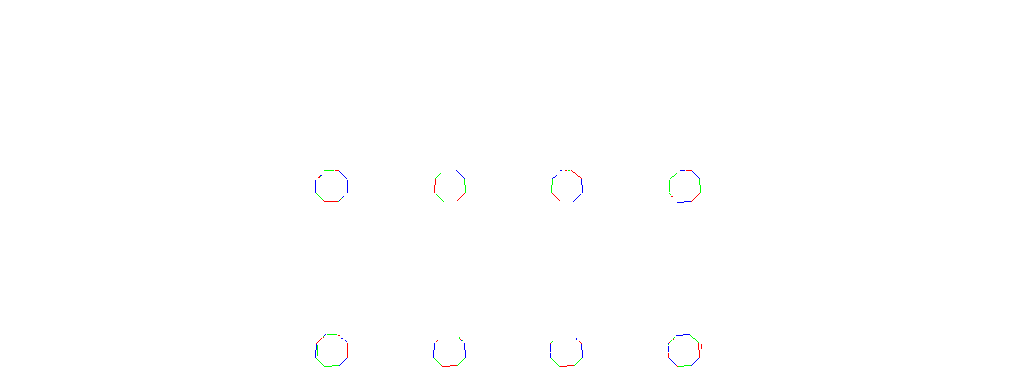
\includegraphics[width=0.13\textwidth]{image_slice_0954_ply.png}} &
\fbox{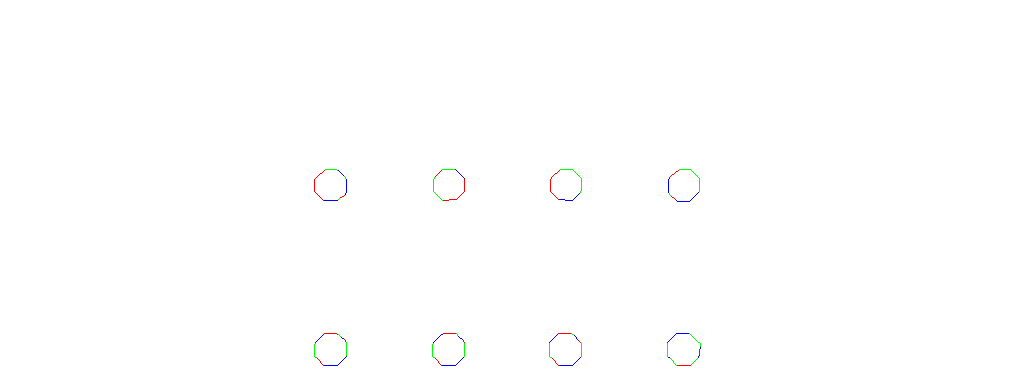
\includegraphics[width=0.13\textwidth]{image_slice_0954_rad_4_and_merged.png}} \\
(a) & (b) & (c) \\
\fbox{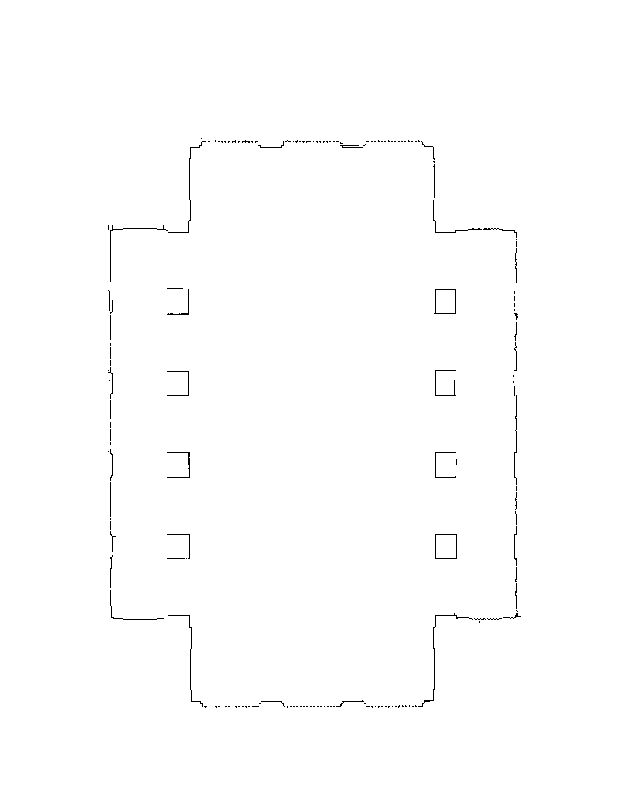
\includegraphics[width=0.13\textwidth]{image_slice_0491_p1.png}} &
\fbox{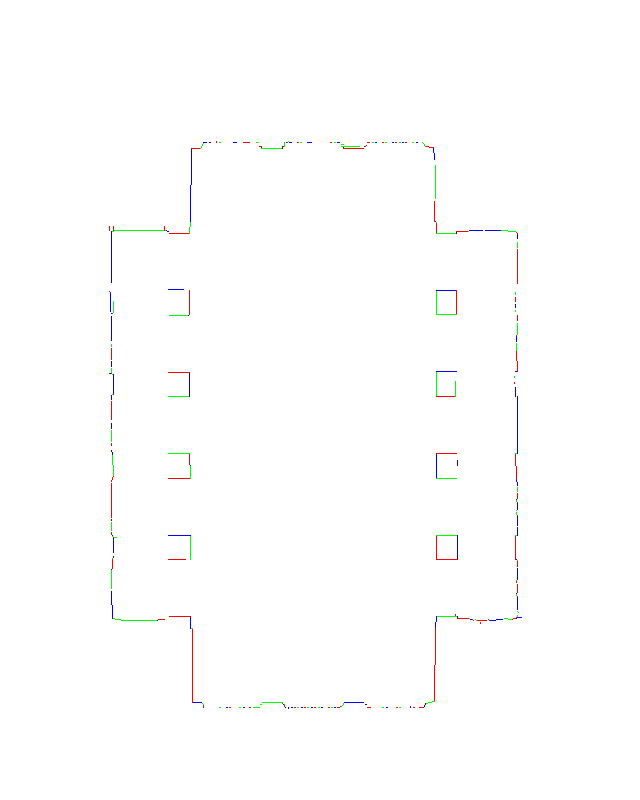
\includegraphics[width=0.13\textwidth]{image_slice_0491_p1_ply.png}} &
\fbox{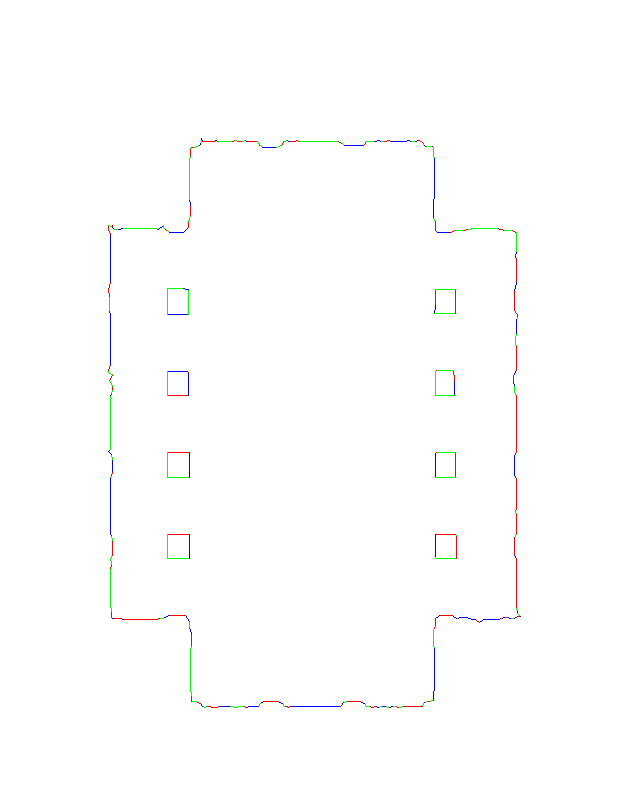
\includegraphics[width=0.13\textwidth]{image_slice_0491_p1_rad_4_and_merged.png}} \\
(d) & (e) & (f) \\
\fbox{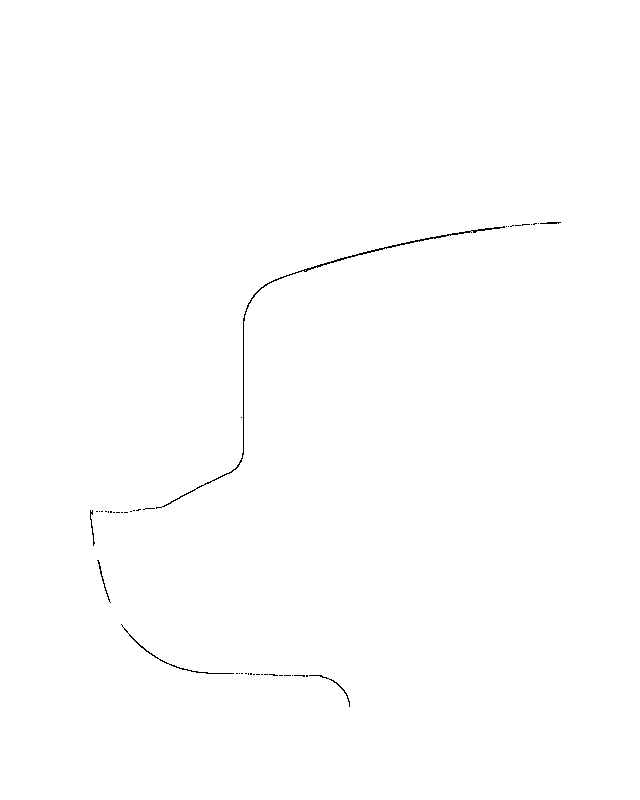
\includegraphics[width=0.13\textwidth]{image_slice_0341.png}} &
\fbox{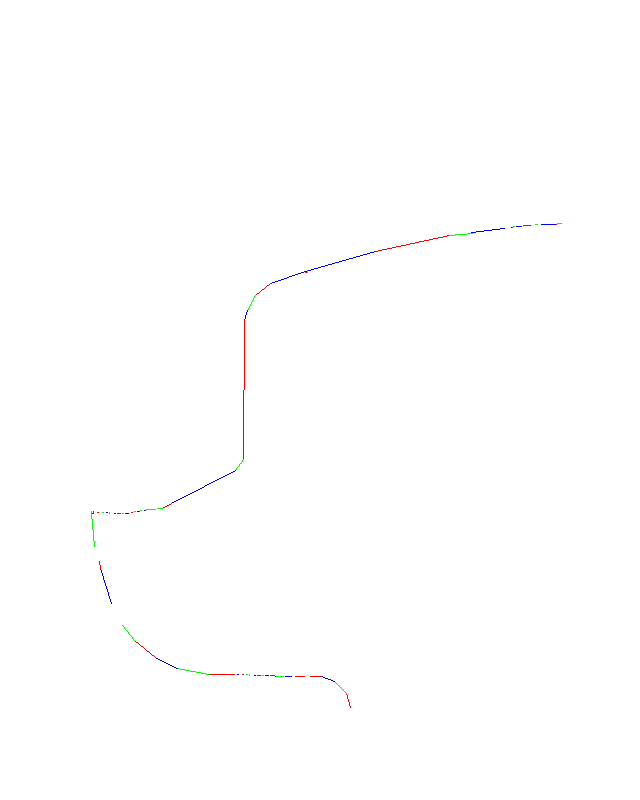
\includegraphics[width=0.13\textwidth]{image_slice_0341_ply.png}} &
\fbox{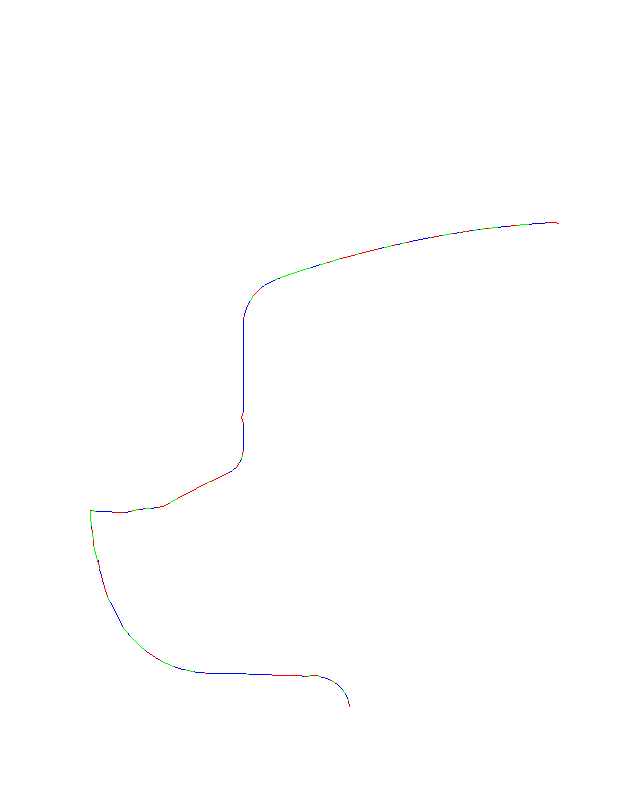
\includegraphics[width=0.13\textwidth]{image_slice_0341_rad_4_and_merged.png}} \\
(g) & (h) & (i) \\
\end{tabular}
\end{center}
\caption{
More experimental results: (a), (d) and (g) show the original noisy binary images.
(b), (e) and (h) show the vectorization results from DP algorithm.
(c), (f) and (i) show the vectorization results from proposed algorithm.}
\label{fig:results}
\end{figure}

%%%%%%%%%%%%%%%%%%%%%%%%%%%%%%%%
%%%%%%   Conclusion and Future Work%%%
%%%%%%%%%%%%%%%%%%%%%%%%%%%%%%%%
\section{Experimental Results}

In addition to the results shown in \Fig{failed_case} and \Fig{HT_BPA_figure}, more
experimental results are shown in \Fig{results}. In the first row of \Fig{results},
the input image is of size 1024x392 and contains multiple contours.
In the second row, the input image is 800x640 and contains nested contours.
In the third row, the input image is 800x640 and contains a curved contour.
As one can see, the proposed framework can handle all the cases properly and fill the holes as expected, which
outperformed the standard DP algorithm.

\section{Conclusion}

An efficient general framework based on 2D ball-pivot algorithm is proposed
for noisy raster image boundary vectorization.
The time and space complexity for this algorithm is $O(n)$.
The proposed method outperformed the existed methods in terms of noise suppression and
holes filling. Various experimental results are showing that the proposed method
can handle all kinds of complicated cases, including nested,
curved and compounded boundaries, etc.

However, there are some limitations for the proposed approach. First, it could
not suppress the noisy data falling outside of the boundary. In fact, it is
sensitive to those noisy data and may introduce some false features due to the noise.
Second, the initial BPA will dominate the following refinement process. Therefore, improper chosen of the
radius for the initial BPA may cause problems for the final results, which may
happen for some extremely complicated raster images.

\section{Acknowledgement}
I would like to thank George Wolberg and Siavash Zokai for their valuable discussions
and suggestions.

%\\
%\\
%\\
%
%KEY POINTS to MAKE:
%
%*. Lift to say that we are proposing a general framework of boundary vectorization:\\
%1. selecting a starting point(scan from left, test the touched point to make sure it
%is not a isolated point, try to put the ball on the data to include only one data point);
%pivoting the ball until: A. reach the starting point. B.
%turning around dectected. 2. refine the boundary to get the details. 3. use a threshold
%to removed detected contour and check whether we need another around of computation.\\
%SHOW RESULTS: closed form, non-closed form, multiple contours form.
%
%*. there are too many vectices in the contour when $\tau_r$ is small,
%so we could apply the algorithm
%of someone who use a minimum vertcies polygon to approximating the original one.
%We do it further by first detection vertices lies on the same line and then by incorporating lines from HT. \\
%SHOW RESULTS: HT beauitfied form
%
%*. The choice of the parameters

%\section{ILLUSTRATIONS, GRAPHS, AND PHOTOGRAPHS}
%\label{sec:illust}
%
%Illustrations must appear within the designated margins.  They may span the two
%columns.  If possible, position illustrations at the top of columns, rather
%than in the middle or at the bottom.  Caption and number every illustration.
%All halftone illustrations must be clear black and white prints.  Colors may be
%used, but they should be selected so as to be readable when printed on a
%black-only printer.
%
%Since there are many ways, often incompatible, of including images (e.g., with
%experimental results) in a LaTeX document, below is an example of how to do
%this \cite{Lamp86}.
%
%% Below is an example of how to insert images. Delete the ``\vspace'' line,
%% uncomment the preceding line ``\centerline...'' and replace ``imageX.ps''
%% with a suitable PostScript file name.
%% -------------------------------------------------------------------------
%\begin{figure}[htb]
%
%\begin{minipage}[b]{1.0\linewidth}
%  \centering
%  \centerline{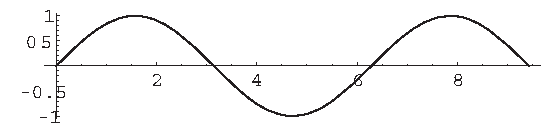
\includegraphics[width=8.5cm]{image1}}
%%  \vspace{2.0cm}
%  \centerline{(a) Result 1}\medskip
%\end{minipage}
%%
%\begin{minipage}[b]{.48\linewidth}
%  \centering
%  \centerline{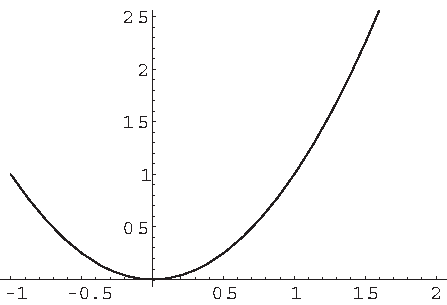
\includegraphics[width=4.0cm]{image3}}
%%  \vspace{1.5cm}
%  \centerline{(b) Results 3}\medskip
%\end{minipage}
%\hfill
%\begin{minipage}[b]{0.48\linewidth}
%  \centering
%  \centerline{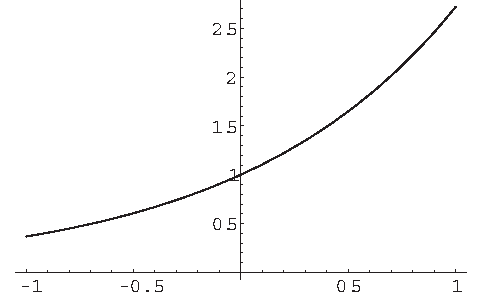
\includegraphics[width=4.0cm]{image4}}
%%  \vspace{1.5cm}
%  \centerline{(c) Result 4}\medskip
%\end{minipage}
%%
%\caption{Example of placing a figure with experimental results.}
%\label{fig:res}
%%
%\end{figure}
%
%
%% To start a new column (but not a new page) and help balance the last-page
%% column length use \vfill\pagebreak.
%% -------------------------------------------------------------------------
%\vfill
%\pagebreak
%
%
%\section{FOOTNOTES}
%\label{sec:foot}
%
%Use footnotes sparingly (or not at all!) and place them at the bottom of the
%column on the page on which they are referenced. Use Times 9-point type,
%single-spaced. To help your readers, avoid using footnotes altogether and
%include necessary peripheral observations in the text (within parentheses, if
%you prefer, as in this sentence).
%
%
%\section{COPYRIGHT FORMS}
%\label{sec:copyright}
%
%You must include your fully completed, signed IEEE copyright release form when
%you submit your paper. We {\bf must} have this form before your paper can be
%published in the proceedings.
%
%\section{REFERENCES}
%\label{sec:ref}
%
%List and number all bibliographical references at the end of the paper.  The references can be numbered in alphabetic order or in order of appearance in the document.  When referring to them in the text, type the corresponding reference number in square brackets as shown at the end of this sentence \cite{C2}.
%
%% References should be produced using the bibtex program from suitable
%% BiBTeX files (here: strings, refs, manuals). The IEEEbib.bst bibliography
%% style file from IEEE produces unsorted bibliography list.
%% -------------------------------------------------------------------------
\bibliographystyle{IEEEbib}
\bibliography{icip}

\end{document}
